\section{Database View}
In this part of the \emph{Design Document} is reported the design and the main entities used by \emph{Travlendar+} System.

\begin{figure}[H]
    \centering
    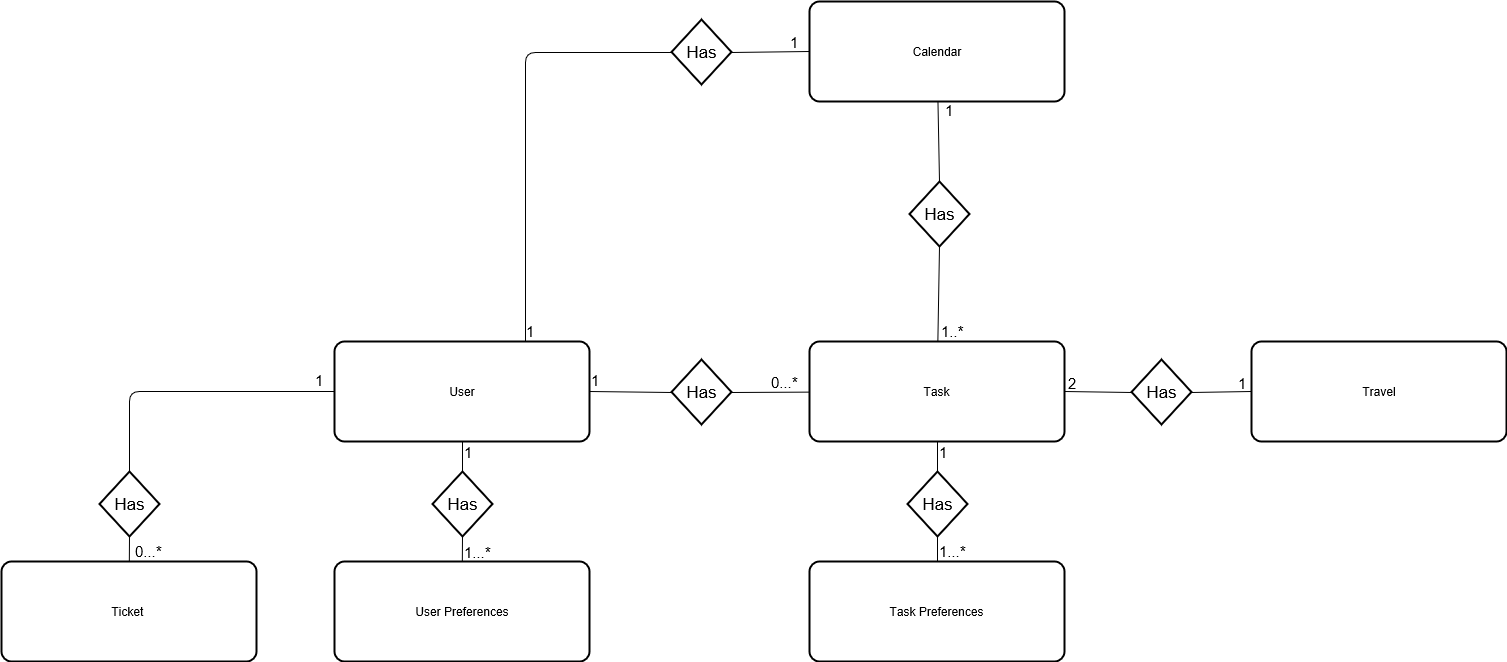
\includegraphics[scale=0.27]{Pictures/DatabaseDiagrams/E-R_Diagram.png}
    \caption{E-R Diagram}
\end{figure}

As can be noticed, the Database is composed by six main entities, useful for the correct behavior of the \emph{Travlendar+} System.

The main entities is the \emph{User} one, that is used to store properly the main information about the user's account into the System, and it is also used for the Log In procedure. An user can have at least one preference, stored in the User Preferences table.
Moreover, to take into account the cost of a travel, the \emph{Travlendar+} System needs to know if the user has some tickets yet, because in this situation the travel cost can be null. For this reason, the system stores also some information about the user's tickets.
Obviously, the user's needs to schedule his calendar, to do that the \emph{Travlendar+} System needs to know the tasks the user has to do, and also their preferences; in this way, the system can compute a feasible calendar for him, and then it stores this calendar into a proper entity in the Database System.

To have more information about the attributes of each tables, here are reported some pictures to explain well this:

\begin{figure}[H]
    \centering
    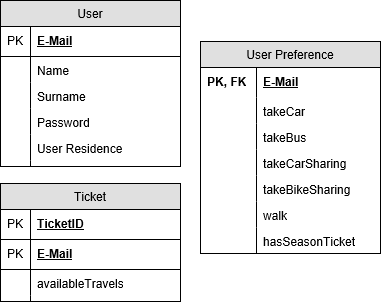
\includegraphics[scale=0.6]{Pictures/DatabaseDiagrams/UserRelatedTables.png}
    \caption{Attributes of the user-related tables}
\end{figure}

\begin{figure}[H]
    \centering
    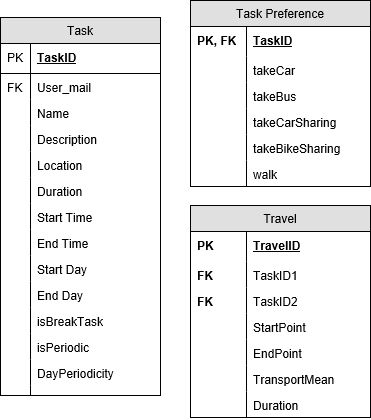
\includegraphics[scale=0.6]{Pictures/DatabaseDiagrams/TaskRelatedTables.png}
    \caption{Attributes of the task-related tables}
\end{figure}

\begin{figure}[H]
    \centering
    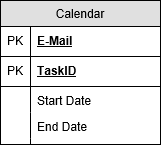
\includegraphics[scale=0.6]{Pictures/DatabaseDiagrams/CalendarRelatedTable.png}
    \caption{Attributes of the calendar-related table}
\end{figure}